\section{Durchführung}
\label{sec:Durchführung}

Die erste Messaufgabe besteht aus der direkten Messung der Leerlaufspannung einer
Monozelle. Dies geschieht über ein hochohmiges Voltmeter. Der Eingangswiderstand
$R_\text{V}$ und die abgelesene Leerlaufspannung werden notiert.
Danach wird die Schaltung mit dem Schaltbild, welches in Abbildung \ref{fig:schaltbild1}
zu sehen ist, aufgebaut.

\begin{figure}
  \centering
  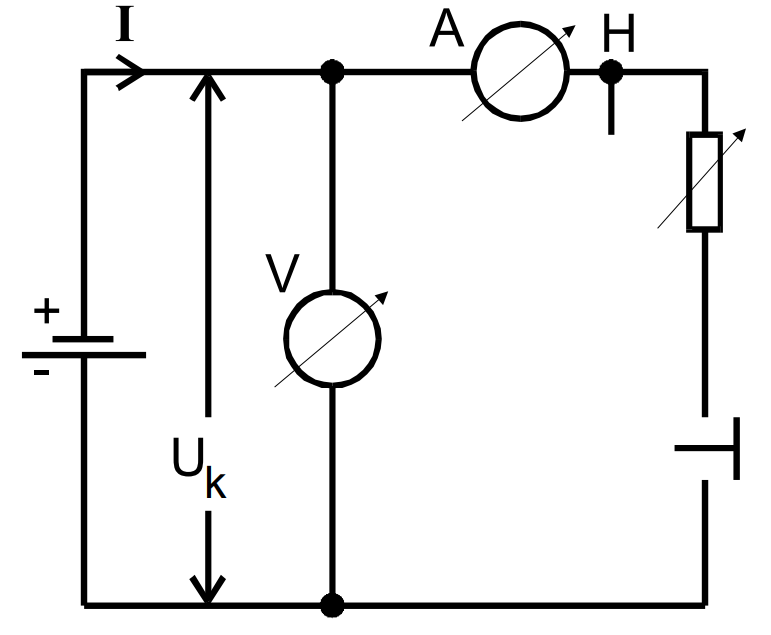
\includegraphics[width=150pt]{data/schaltbild1.png}
  \caption{Schaltbild zur Reihenschaltung einer realen Spannungsquelle mit einer Last und Messgeräten \cite{Versuchsanleitung}}
  \label{fig:schaltbild1}
\end{figure}

Der Lastwiderstand $R_\text{a}$ ist dabei in einem Bereich von $0$ bis
$\SI{50}{\ohm}$ regelbar. Über die Variation des Lastwiderstand wird die Stromstärke,
welche durch das vor den Lastwiderstand geschaltete Amperemeter gemessen wird,
verändert. Dadurch lässt sich die Klemmenspannung $U_\text{K}$ in Abhängkeit der
Stromstärke $I$ aufnehmen.

Nun wird hinter den regelbaren Widerstand eine Gegenspannung geschaltet, welche
ungefähr $\SI{2}{\volt}$ über der bereits näherungsweise gemessenen Leerlaufspannung
liegt. Dies ist in Abbildung \ref{fig:schaltbild2} veranschaulicht.

\begin{figure}
  \centering
  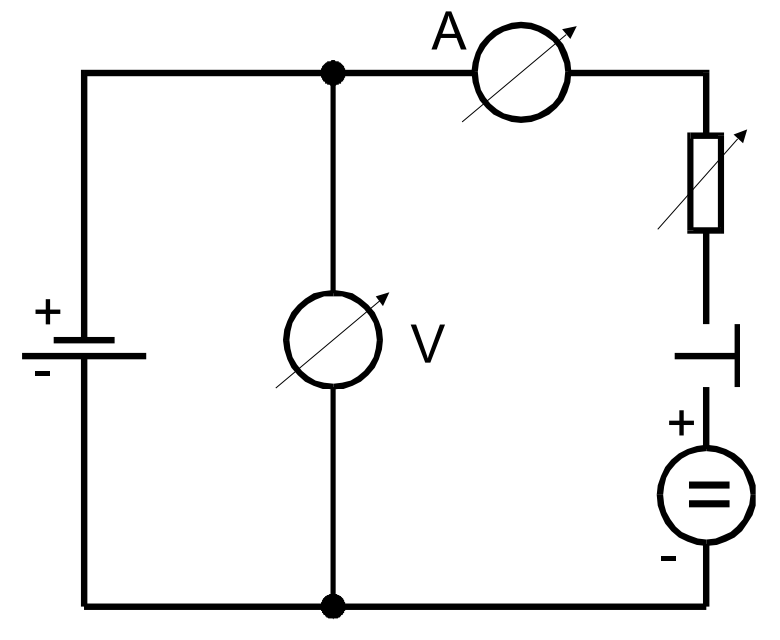
\includegraphics[width=150pt]{data/schaltbild2.png}
  \caption{Schaltbild zur gleichen Schaltung, jedoch mit einer Gegenspannung \cite{Versuchsanleitung}}
  \label{fig:schaltbild2}
\end{figure}

Bei diesem Aufbau erfolgt die Aufnahme der Messwerte genau so wie zuvor beschrieben.

Zuletzt sind Messreihen mit dem Aufbau in Abbildung \ref{fig:schaltbild1} für
Wechselspanungsquellen aufzunehmen. Diese sind ein 1\,V-Rechteckausgang und ein
1\,V-Sinusausgang. Die Lastwiderstände sind erneut regelbar. Für die Rechteckspannung
wird ein Widerstand im Bereich von $\SI{20}{\ohm}$ bis $\SI{250}{\ohm}$
verwendet, für die Sinusspannung gilt der Bereich von $\SI{0.1}{\kilo\ohm}$ bis
$\SI{5}{\kilo\ohm}$.
Außerdem ist auf die Frequenzeichung der Messgeräte zu achten. Die Frequenz der
Wechselspannung ist dieser anzupassen.
